Data-driven science has produced massive datasets from high-throughput instruments, large simulations, and pervasive sensing \cite{noauthororeditorfourth, liew_scientific_2017}, which require sophisticated computational methods.
Scientific workflows are a key abstraction for structuring these computations~\cite{vivas_trends_2024}. Scientific Workflow Management Systems (SWMSs) such as Snakemake~\cite{molder_sustainable_2021} and Nextflow~\cite{di_tommaso_nextflow_2017} let researchers define complex multi-step analyses in a modular and reproducible way.
Because these workflows process large and complex datasets, they require substantial compute, storage, and networking resources \cite{ahmad_scientific_2021}. 
At scale, they may contain hundreds or thousands of jobs and run from hours to months \cite{juve_characterizing_2013, ferreira_da_silva_characterizing_2020}, typically relying on distributed infrastructures such as clusters, grids or clouds~\cite{liu_survey_2015, siar_offloading_2021}.

In heterogeneous compute environments, resources may be geographically and administratively distributed. Such settings introduce non-trivial scheduling and job allocation challenges, which have been addressed by numerous algorithms targeting different performance objectives \cite{shukla_fat-eto_2023,siar_offloading_2021,de_maio_multi-objective_2020,zhang_task_2017,wang_energy-efficient_2019,kaur_focalb_2021}. A widely used approach, particularly in the cloud-continuum, is job offloading between available compute environments to satisfy user-defined objectives \cite{khan_fog_2017,mcc}.
Although workflow scheduling and resource allocation within single clusters have been extensively investigated, a single cluster can still be insufficient to satisfy the resource or time requirements of large-scale workflows. Especially long-running workflows can monopolize cluster resources and delay result availability. Users often require faster turnaround times and may therefore rely on secondary resources to meet time constraints. In such cases, the systematic offloading of jobs to alternative clusters can alleviate resource contention and thereby improve overall workflow makespan.
Motivated by this scenario, this work extends the concept of job offloading to the execution of scientific workflows in distributed multi-cluster environments \cite{hutchison_mip_2013}.

\begin{figure}[t]
    \centering
    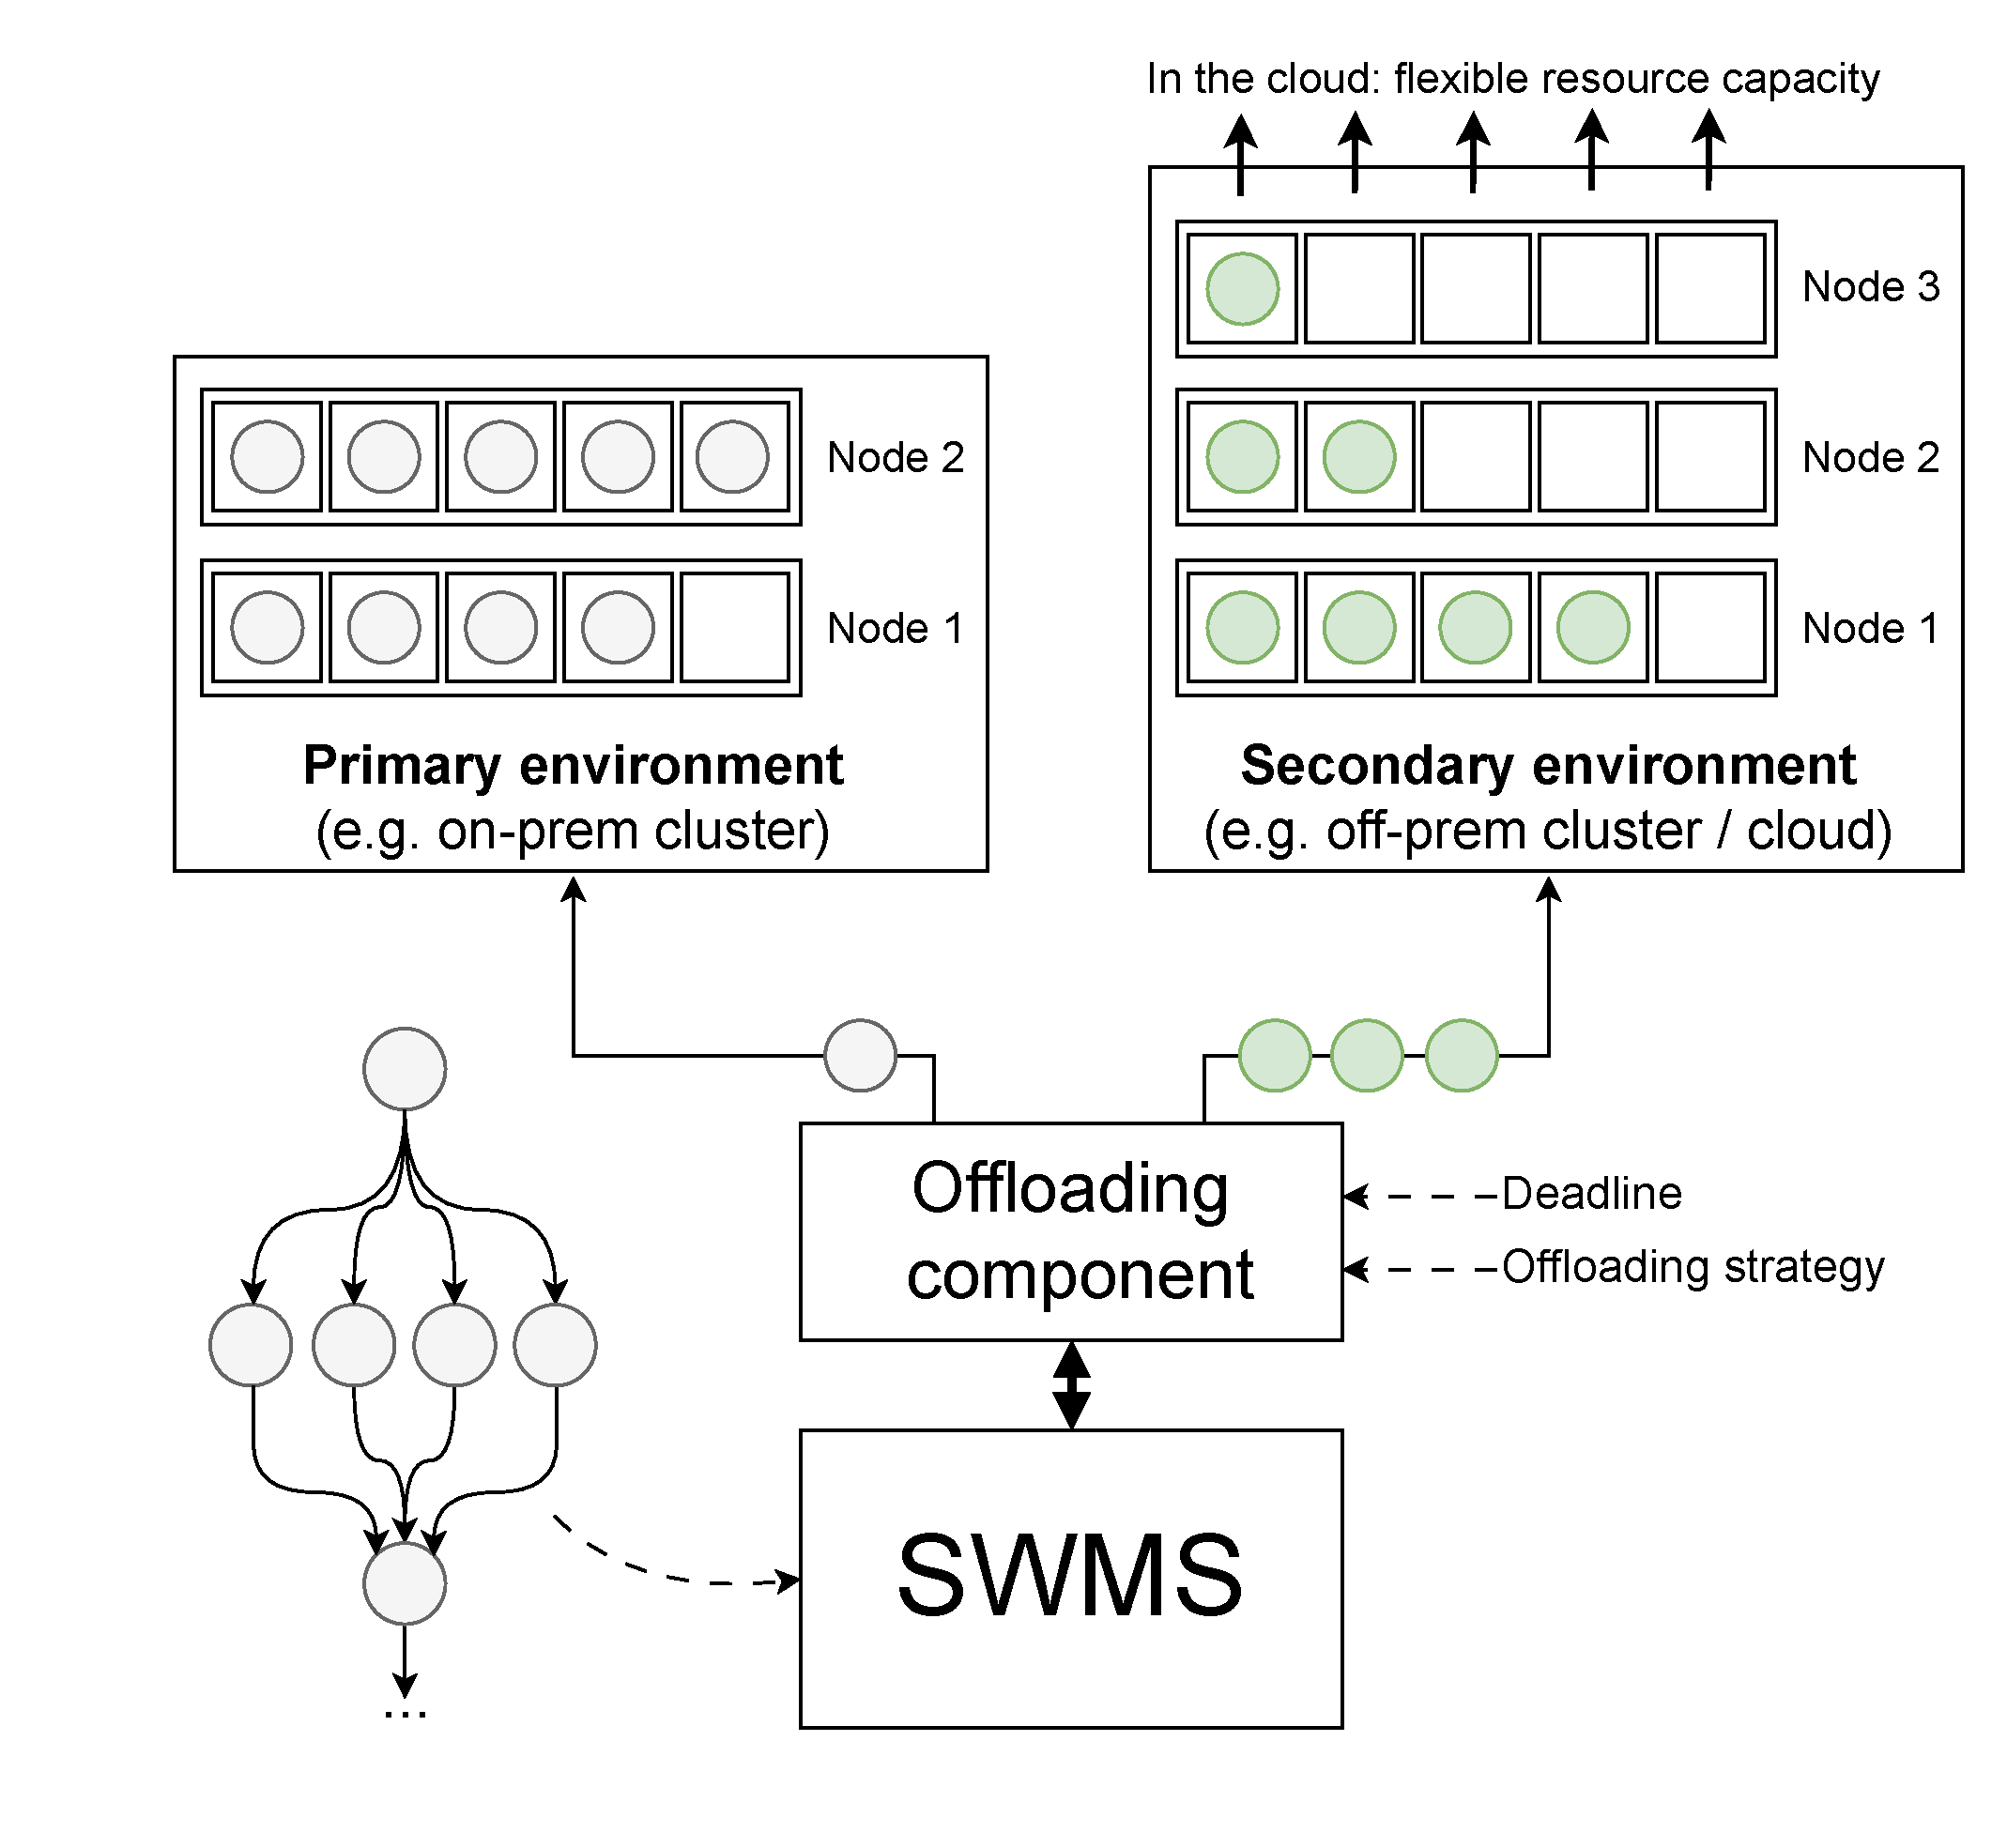
\includegraphics[width=1\linewidth]{./img/idea_introduction_smaller.drawio.pdf}
    \caption{Overview of the multi-cluster offloading problem for scientific workflows}
    \label{fig:intro}
\end{figure}

Fig.~\ref{fig:intro} illustrates the offloading scenario we consider in this paper. We assume a primary compute environment that serves as the default execution site, but may be unable to satisfy workflow deadlines due to limited resource capacity. To address this limitation, a secondary environment is available that can provide additional resources when necessary. 

All jobs are executed in the primary environment unless offloading is explicitly performed. A typical primary environment is an on-premise cluster that is readily accessible to users, provides limited computational capacity, and does not incur direct monetary cost. The secondary environment serves as an alternative execution site to which selected jobs can be offloaded. In practice, this secondary environment can correspond to an off-premise cluster with restricted capacity or to a cloud platform that offers resources on demand.

 As in many practical scenarios, particularly when using cloud resources, offloading introduces monetary costs proportional to the consumed resources and execution time. Therefore, the use of secondary environments must remain economically feasible, requiring careful control of offloading decisions. 

In this work, we propose the design and implementation of an offloading component that interacts with the SWMS to guide the workflow execution by determining which jobs should be offloaded to a secondary environment. This component is plugged into the SWMS and takes as input a user-defined deadline for the overall workflow makespan, as well as an offloading strategy \cite{ahmad_scientific_2021}.

The paper makes the following contributions:
\begin{enumerate}
  \item We propose a heuristic two-step approach: (i) predict job runtimes using linear models trained on historical data, and (ii) simulate workflow execution on multi-clusters using these predictions to select jobs for offloading that meet user-defined deadlines while minimizing cost.
  \item We provide our implementation as an extension to the Snakemake SWMS. The source code and the workflow execution data collected during our experiments are made publicly available.\footnote{{published after acceptance.}}
\end{enumerate}

